\documentclass[letterpaper,11pt]{article}
\oddsidemargin -1.0cm \textwidth 17.5cm

\usepackage[utf8]{inputenc}
\usepackage[activeacute,spanish]{babel}
\usepackage{amsfonts,setspace}
\usepackage{amsmath}
\usepackage{amssymb, amsmath, amsthm}
\usepackage{comment}
\usepackage{amssymb}
\usepackage{dsfont}
\usepackage{anysize}
\usepackage{multicol}
\usepackage{enumerate}
\usepackage{graphicx}
\usepackage[left=1.5cm,top=2cm,right=1.5cm, bottom=1.7cm]{geometry}
\setlength\headheight{1.5em} 
\usepackage{fancyhdr}
\usepackage{multicol}
\usepackage{hyperref}
\usepackage{wrapfig}
\pagestyle{fancy}
\fancyhf{}
\renewcommand{\labelenumi}{\normalsize\bfseries P\arabic{enumi}.}
\renewcommand{\labelenumii}{\normalsize\bfseries (\alph{enumii})}
\renewcommand{\labelenumiii}{\normalsize\bfseries \roman{enumiii})}

\begin{document}

\fancyhead[L]{\itshape{Facultad de Ciencias F\'isicas y Matem\'aticas}}
\fancyhead[R]{\itshape{Universidad de Chile}}

\begin{minipage}{11.5cm}
    \begin{flushleft}
        \hspace*{-0.6cm}\textbf{FI1000-5 Introducción a la Física Clásica}\\
        \hspace*{-0.6cm}\textbf{Profesora:} Paulina Lira\\
        \hspace*{-0.6cm}\textbf{Auxiliares:} Alejandro Silva, Felipe Kaschel, Juan Cristobal Castro\\
    \end{flushleft}
\end{minipage}

\begin{picture}(2,3)
    \put(405,-5){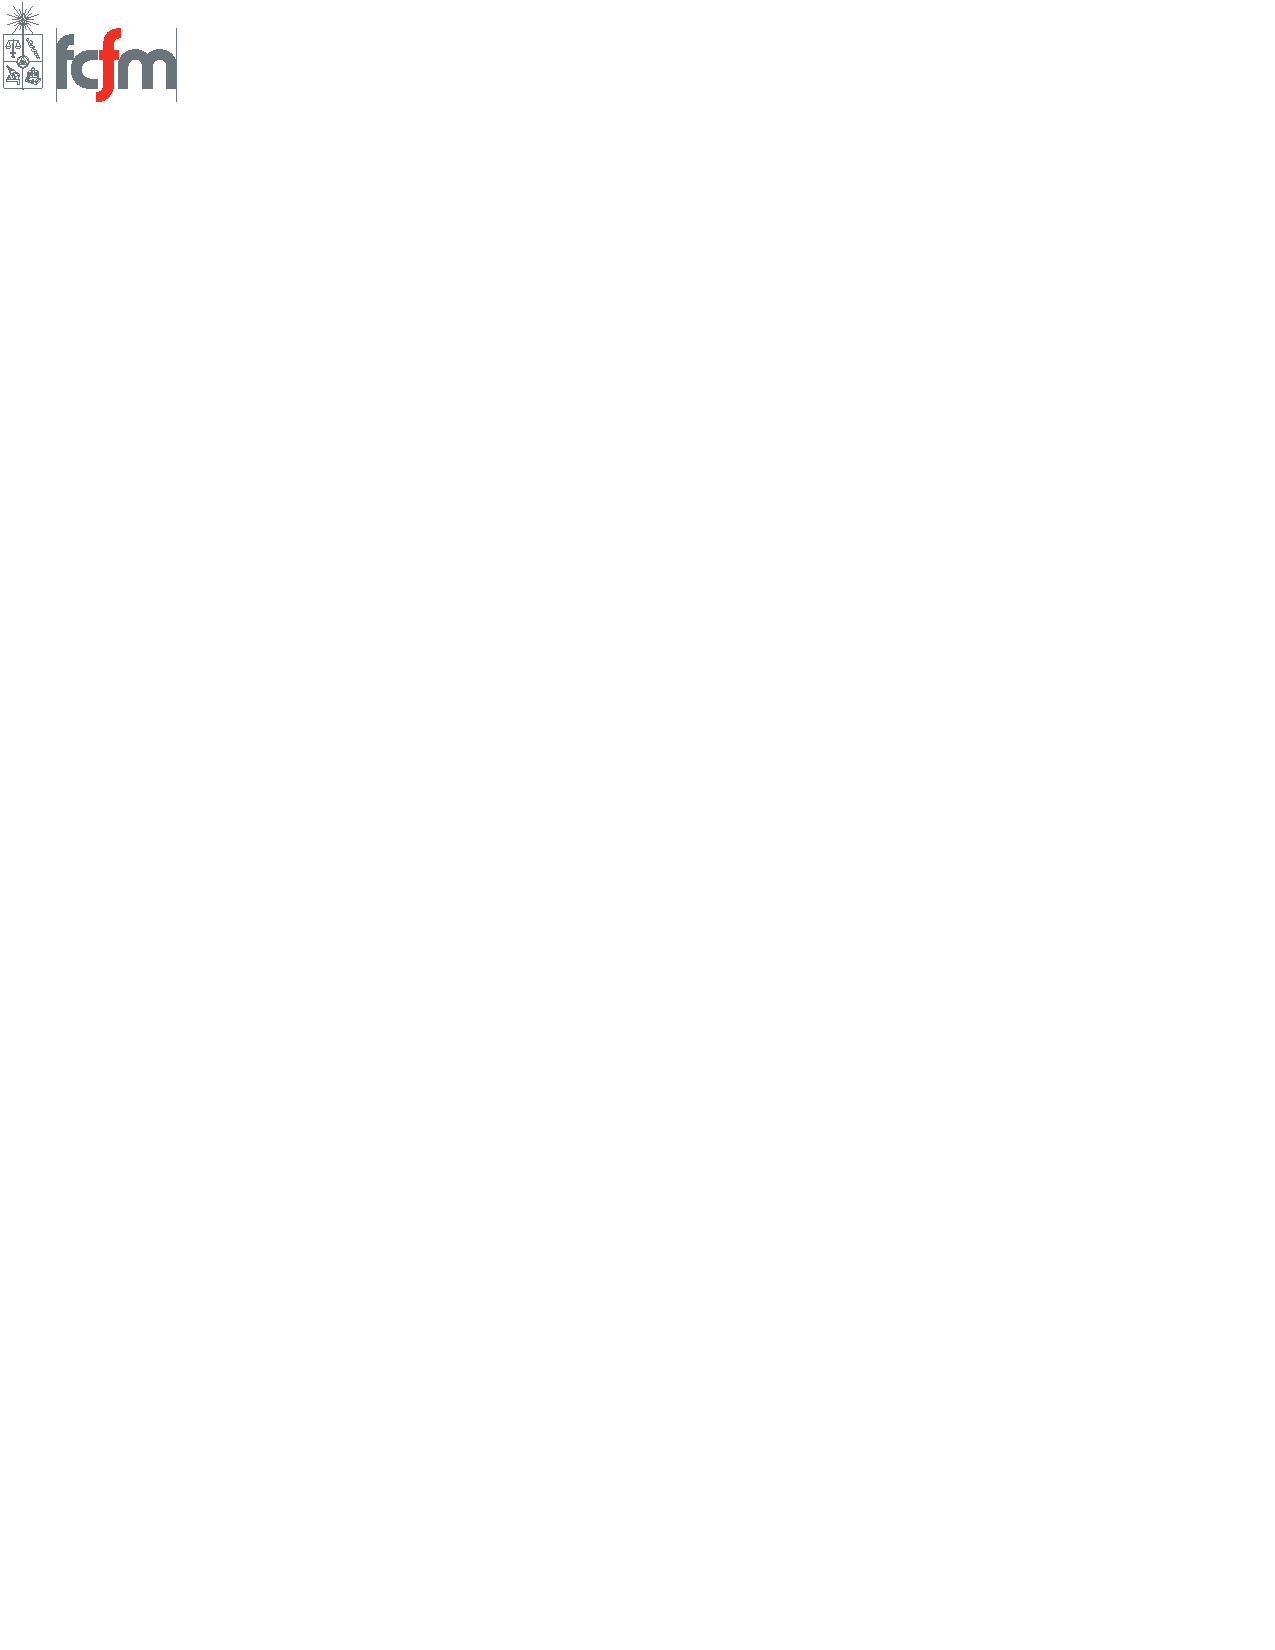
\includegraphics[scale=1.25]{2020-1/Imágenes/logo/fcfm2.pdf}}
\end{picture}

\begin{center}
	\LARGE \bf Auxiliar \#9: Preparación C1   \\
\end{center}

\vspace{-1cm}
\begin{enumerate}\setlength{\itemsep}{0.4cm}

\rfoot[]{pág. \thepage}

\item[]

\item $P4$, CONTROL 2, $2005$. Dos planetas de masas $m_1$ y $m_2$ giran en órbitas circulares de radio $r_1$ y $r_2$ respectivamente, en torno a un astro de masa M$>>>m_1$,$m_2$. Desprecie la interacción gravitacional entre las masas pequeñas y encuentre la constante de rigidez $k$ de un resorte que, unido a ambos planetas en la configuración que se muestra en la figura, logre que giren con el mismo periodo. Considere que el resorte tiene masa despreciable y largo natural nulo. \\

\begin{figure}[h!]
        \centering
        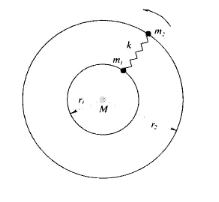
\includegraphics[scale=1]{2020-1/Imágenes/aux9/imagen p1 aux9.png}
    \end{figure}


\item P3- CONTROL 1 - 2005  Una particula de masa $m$ está unida a dos cuerdas ideales de igual largo L. Los extremos libres de ambas cuerdas se unen a una barra vertical, separads por una distancia L. Si la barra gira en torno a su eje con rapidez angular constante $w$ de manera que ambas cuerdas estén tensas:

i) determine la tensión de cada una de las cuerdas

ii) Encuentre la rapidez angular mínima que se requiere para que efectivamente ambas cuerdas estén tensas.
    
   \begin{figure}[h!]
        \centering
        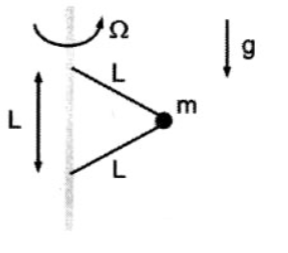
\includegraphics[scale=1
        ]{2020-1/Imágenes/aux9/p2a9}
    \end{figure} 
    
\newpage
    
\item  P3 - CONTROL 2- 2007   Un resorte de constante elástica $k$ y largo natular $L_o = (\pi*R)/2$ se enrolla en un aro de radio $R$. Uno de los extremos del resorte está fijo al aro en el punto $O$ mientras que el otro extremo está unido a una argolla de masa $m$ que desliza sin roce por el aro. El conjunto se monta sobre una plataforma que se mueve sin roce sobre un plano horizontal. Producto de la aceleración de la plataforma, el resorte se estira. Determine la aceleración de la plataforma $a_o$ cuando la posición de la argolla m está dada por un ángulo $\theta$ con respecto a la vertical.   \\

        
    \end{enumerate}
    
       \begin{figure}[h!]
        \centering
        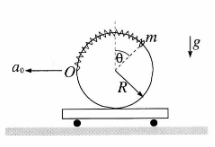
\includegraphics[scale=1
        ]{2020-1/Imágenes/aux9/p3a9}
    \end{figure} 

\end{enumerate}
\end{document}